\documentclass[10pt, a4paper]{article}
\usepackage[utf8]{inputenc}
\usepackage[T1]{fontenc,url}
\usepackage{multicol}
\usepackage{multirow}
\usepackage{parskip}
\usepackage{lmodern}
\usepackage{microtype}
\usepackage{verbatim}
\usepackage{amsmath, amssymb}
\usepackage{tikz}
\usepackage{physics}
\usepackage{mathtools}
\usepackage{algorithm}
\usepackage{algpseudocode}
\usepackage{listings}
\usepackage{enumerate}
\usepackage{graphicx}
\usepackage{float}
\usepackage{hyperref}
\usepackage{tabularx}
\usepackage{siunitx}
\usepackage{fancyvrb}
%\usepackage{natbib}
%\bibliographystyle{dinat}
\usepackage[makeroom]{cancel}
\usepackage[margin=2.0cm]{geometry}
\usepackage{pdfpages}
\usepackage[margin=10pt, textfont={small, it}, labelfont={bf}, labelsep=endash]{caption}
\renewcommand{\baselinestretch}{1}
\renewcommand{\exp}{e^}
\renewcommand{\b}{\boldsymbol}
\newcommand{\h}{\hat}
\newcommand{\m}{\mathbb}
\newcommand{\half}{\frac{1}{2}}
\renewcommand{\exp}{e^}
\renewcommand{\bar}{\overline}
\setlength\parindent{0pt}


\begin{document}
\title{AST5220\\ Milestone II -- Recombination}
\author{
    \begin{tabular}{r l}
        Jonas Gahr Sturtzel Lunde & (\texttt{jonassl})
    \end{tabular}}
% \date{}    % if commented out, the date is set to the current date

\maketitle
Code found at \url{https://github.com/asdfbat/AST5220/tree/master/Project}
\vspace{0.7cm}

\section{Theory}

\subsection{Dimensionality analysis}
We introduce the following notation
\begin{itemize}
    \item $T$ - Temperature
    \item $t$ - Time
    \item $M$ - Mass
    \item $L$ - Length
    \item $E$ - Energy ($E = ML^2t^{-2}$)
\end{itemize}

In natural units, quantities are scaled in such a way that $c = \hbar = k_B = 1$. The dimensions of these three constants are
\begin{itemize}
    \item $[c] = Lt^{-1}$
    \item $[\hbar] = Et = ML^2t^{-1}$
    \item $[k_B] = ET^{-1} = ML^2t^{-2}T^{-1}$
\end{itemize}

\subsection{Saha equation dimensionality analysis}
\begin{equation}
    \frac{X_{e}^{2}}{1-X_{e}}= \underbrace{\frac{1}{n_{b}}\qty(\frac{m_{e} T_{b}}{2 \pi})^{3 / 2} e^{-\epsilon_{0} / T_{b}}}_A
\end{equation}

Exponents are not physically allowed to be unitless, and the exponent in the last term in the Saha equation must therefore lacks one or more constants. We quickly see that multiplying the temperature in the divisor with $k_B$ gives the divisor units of energy. This cancels the units of energy in the dividend, making the exponent unitless.

The left-hand side(LHS) of the Saha equation is unitless (as $X_e$ is unitless), meaning the left-hand side(LHS), which we've named $A$, must be unitless as well. A initially contain dimensions of
\begin{equation*}
    [A] = [n_b^{-1}][m_e^{3/2}][T_b^{3/2}] = L^3M^{3/2}T^{3/2}
\end{equation*}
We need a combination of $\hbar$, $c$ and $k_B$ which removes these dimensions. We observe that the dimensions of temperature must be removed by a factor of $k_B^{3/2}$, as no other of the constants contains dimensions of temperature. We're then left with the units of
\begin{equation*}
    [A][k_B^{3/2}] = L^6M^3t^{-3}
\end{equation*}
We immediately recognize this as the units of $\hbar^3$, meaning that multiplying by the factor of $\hbar^{-3}$ will make A a unitless quantity. The Saha expression with all relevant constants then reads
\begin{equation}\label{eqn:Saha}
    \frac{X_{e}^{2}}{1-X_{e}} = A\ , \quad A = \frac{1}{n_{b}\hbar^3}\qty(\frac{m_{e} k_B T_{b}}{2 \pi})^{3 / 2} e^{-\epsilon_{0} / k_B T_{b}}
\end{equation}


\subsection{Peebles equation dimensionality analysis}

\begin{equation}
    \label{eqn:Peebles}
    \dv{X_{e}}{x}=\frac{C_{r}\qty(T_{b})}{H}\qty[\beta\qty(T_{b})\qty(1-X_{e})-n_{H} \alpha^{(2)}\qty(T_{b}) X_{e}^{2}]
\end{equation}

\begin{align}
    \label{eqn:1}
    C_{r}\qty(T_{b}) &=\frac{\Lambda_{2 s \rightarrow 1 s}+\Lambda_{\alpha}}{\Lambda_{2 s \rightarrow 1 s}+\Lambda_{\alpha}+\beta^{(2)}\qty(T_{b})} \\
    \label{eqn:2}
    \Lambda_{2 s \rightarrow 1 s} &=8.227 \mathrm{s}^{-1} \\
    \label{eqn:4}
    \Lambda_{\alpha} &=H \frac{\qty(3 \epsilon_{0})^{3}}{(8 \pi)^{2} n_{1 s}} \\
    \label{eqn:5}
    n_{1 s} &=\qty(1-X_{e}) n_{H} \\
    \label{eqn:6}
    \beta^{(2)}\qty(T_{b}) &=\beta\qty(T_{b}) e^{3 \epsilon_{0} / 4 T_{b}} \\
    \label{eqn:7}
    \beta\qty(T_{b}) &=\alpha^{(2)}\qty(T_{b})\qty(\frac{m_{e} T_{b}}{2 \pi})^{3 / 2} e^{-\epsilon_{0} / T_{b}} \\
    \label{eqn:8}
    \alpha^{(2)}\qty(T_{b}) &=\frac{64 \pi}{\sqrt{27 \pi}} \frac{\alpha^{2}}{m_{e}^{2}} \sqrt{\frac{\epsilon_{0}}{T_{b}}} \phi_{2}\qty(T_{b}) \\
    \label{eqn:9}
    \phi_{2}\qty(T_{b}) &=0.448 \ln \qty(\epsilon_{0} / T_{b})
\end{align}



\subsubsection{\texorpdfstring{$\mathbf{n_{1s}}$}{TEXT} }
Starting with the most trivial case, the relative density of 1s Hydrogen, $n_{1s}$ carries the units of $L^{-3}$ from the hydrogen number density $n_H$. Since this is the correct units for a number density, we leave it unchanged.


\subsubsection{\texorpdfstring{$\mathbf{\phi_2(T_b)}$}{TEXT} }
The logarithmic term in $\phi_2(T_b)$ must produce a unitless quantity. Multiplying the temperature $T_b$ with $k_B$ gives the divisor units of energy, making the logarithm unitless. The correct expression for $\phi_2(T_b)$ is then
\begin{equation*}
    \phi_{2}\qty(T_{b}) = 0.448 \ln \qty(\epsilon_{0} / k_b T_{b})
\end{equation*}

\subsubsection{\texorpdfstring{$\mathbf{\Lambda_{2s\rightarrow1s}}$}{TEXT} }
$\Lambda_{2s\rightarrow1s}$ is the transition rate of the $2s\rightarrow 1s$ transition in a Hydrogen atom. A transition rate should have dimensions of $t^{-1}$, which it has.

In expression \ref{eqn:1}, $\Lambda_{2s\rightarrow1s}$ is added to the quantities $\Lambda_\alpha$ and $\beta^{(2)}$. These two quantities must therefore also have units of $t^{-1}$.

\subsubsection{\texorpdfstring{$\mathbf{\Lambda_\alpha}$}{TEXT} }
$\Lambda_\alpha$ should have units of $t^{-1}$. In our initial expression, it has units of
\begin{equation*}
    \qty[\Lambda_\alpha] = [H][\epsilon_0][n_H^{-1}] = t^{-1}E^3L^3
\end{equation*}
We need something with units $(EL)^{-3}$ in order to get $\Lambda_\alpha$ to the right units. We can easily observe that $[c][\hbar] = EL$, such that $[c\hbar^{-3}] = (EL)^{-3}$ The correct expression for $\Lambda_\alpha$ therefore reads
\begin{equation*}
    \Lambda_{\alpha} =H \frac{\qty(3 \epsilon_{0})^{3}}{(8 \pi)^{2} (c\hbar)^3 n_{1 s}}
\end{equation*}

\subsubsection{\texorpdfstring{$\mathbf{\beta^{(2)}}$}{TEXT} }
The exponent in $\beta^{(2)}$ needs to be unitless. Multiplying the temperature $T_b$ with $k_B$ will give it units of energy, making the exponent unitless. Apart from that, $\beta^{(2)}$ simply constraints $\beta$ to have units of $t^{-1}$. The correct expression for $\beta^{(2)}$ is therefore simply
\begin{equation*}
    \beta^{(2)}\qty(T_{b}) =\beta\qty(T_{b}) e^{3 \epsilon_{0} / 4 k_B T_{b}}
\end{equation*}

\subsubsection{\texorpdfstring{$\mathbf{C_r(T_b)}$}{TEXT} }
Since $\beta$ further depends on $\alpha^{(2)}$, the constraints so far would leave ambiguity as to where constants should be placed. We therefore take a look at the Peebles equation \ref{eqn:Peebles}. The right hand side is unitless, meaning the left hand side must be too. If we write out the brackets, each term must be unitless. The left term has units of
\begin{equation*}
    [C_r(T_b)][H^{-1}][\beta] = [C_r(T_b)]t\cdot t^{-1} = [C_r(T_b)] = (unitless)
\end{equation*}
The equation for $C_r(T_b)$ can therefore be left unchanged. It is already unitless, as it should.

\subsubsection{\texorpdfstring{$\mathbf{\alpha^{(2)}}$}{TEXT} }
Following the same logic as above, the right term on the right hand side of the Peebles equation must be unitless. We can therefore make the following constraint:
\begin{equation*}
    [H^{-1}][n_H][\alpha^{(2)}] = tL^{-3}[\alpha^{(2)}] = (unitless) \quad\Rightarrow\quad [\alpha^{(2)}] = L^3t^{-1}
\end{equation*}
We know $\phi_2$ and the fine structure constant $\alpha$ to be unitless, meaning our initial expression for $\alpha^{(2)}$ has units of
\begin{equation*}
    [\alpha^{(2)}] = [m_e^{-2}][\epsilon_0^{1/2}][T_b^{-1/2}] = M^{-2}E^{1/2}T^{-1/2}
\end{equation*}
Our only constant containing temperature is $k_B$, meaning the dimension of temperature must be removed by a factor of $k_B$. Multiplying by $k_B^{-1/2}$ removes both the dimensions of energy and temperature, none of which is supposed to be in the final expression. We're then left with
\begin{equation*}
    [\alpha^{(2)}][k_B^{1/2}] = M^{-2}
\end{equation*}
The remainding work must be done by combinations of $c$ and $\hbar$, as not to reintroduce temperature. It's not hard to see that this can be achived by
\begin{equation*}
    [\hbar^n][c^m] = L^3t^{-1}M^2  \quad\Rightarrow\quad n=2,\ m=-1
\end{equation*}

$\alpha^{(2)}$ now reads
\begin{equation*}
    \alpha^{(2)}\qty(T_{b}) = \frac{64 \pi}{\sqrt{27 \pi}} \frac{\alpha^{2} \hbar^2}{m_{e}^{2} c} \sqrt{\frac{\epsilon_{0}}{k_B T_{b}}} \phi_{2}\qty(T_{b})
\end{equation*}

Inserting for the Thompson cross-section $\sigma_T$, we get our final expression for $\alpha^{(2)}$.
\begin{equation*}
    \alpha^{(2)}\qty(T_{b}) = \frac{8}{\sqrt{3 \pi}} \sigma_T c \sqrt{\frac{\epsilon_{0}}{k_B T_{b}}} \phi_{2}\qty(T_{b}), \quad \sigma_{T}=\frac{8 \pi}{3} \frac{\alpha^{2} \hbar^{2}}{m_{e}^{2} c^{2}}
\end{equation*}

\subsubsection{\texorpdfstring{\textbf{$\beta$}}{TEXT} }
Now that the units of $\alpha^{(2)}$ is known, the units of $\beta$ is no longer ambiguous. As previous stated, $\beta$ is constrained to have units of $t^{-1}$. In our initial expression, it has units of
\begin{equation*}
    [\beta] = [\alpha^{(2)}][m_e^{3/2}][T_b^{3/2}] = L^3t^{-1}M^{3/2}T^{3/2}
\end{equation*}
As before, the only way of getting rid of temperature is $k_B$, meaning that $\beta$ must at least contain a factor of $k_B^{3/2}$, giving new units of
\begin{equation*}
    [\beta][k_B^{3/2}] = L^6t^{-4}M^3
\end{equation*}
In order to achive dimensions of $t^{-1}$, we need a factor which holds units of $L^{-6}t^{-3}M^3 = (L^2t^{-1}M)^{-3}$. We recognize the units inside the paranthesis to be the units of $\hbar$, meaning that $\beta$ needs a factor of $\hbar^{-3}$ to have the right units.

The exponential term in $\beta$ needs to unitless. This is, again, achived by multiplying the temperature term by $k_B$.

The correct expression for $\beta$ is then
\begin{equation*}
    \beta\qty(T_{b}) = \alpha^{(2)}\qty(T_{b}) \qty(\frac{m_{e} k_B T_{b}}{2 \pi \hbar^2})^{3 / 2} e^{-\epsilon_{0} / k_BT_{b}}
\end{equation*}


\subsection{Solving the Saha equation}
The Saha equation \ref{eqn:Saha} is actually analytically solvable. Multiplying by $(1-X_e)$ on both sides and reshuffling gives us
\begin{equation*}
    \frac{X_e^2}{(1-X_e)} = A \quad \Rightarrow \quad X_e^2 + AX_e - A = 0
\end{equation*}
which is simply a second order equation in $X_e$, with solutions
\begin{equation*}
    X_e = - \frac{A}{2} \pm \frac{1}{2}\qty(A^2 + 4A)^{1/2}
\end{equation*}
The free electron fraction can't physically be negative. The positive solution reads
\begin{equation}\label{eqn:Saha_sol}
    X_e = - \frac{A}{2} + \frac{A}{2}\qty(1 + \frac{4}{A})^{1/2}
\end{equation}

We can also observe from \ref{eqn:Saha} that, as $X_e \rightarrow 1$, A will quickly converge towards zero as $A \propto X_e^2$. This will present a problem for equation \ref{eqn:Saha_sol}, as the $\frac{4}{A}$ term will diverge to infinity.

At the other end, as $X_e \rightarrow 1$, A will diverge to infinity, as $A \propto X_e^{-1}$.


\section{Results}
\begin{figure}[H]
    \centering
    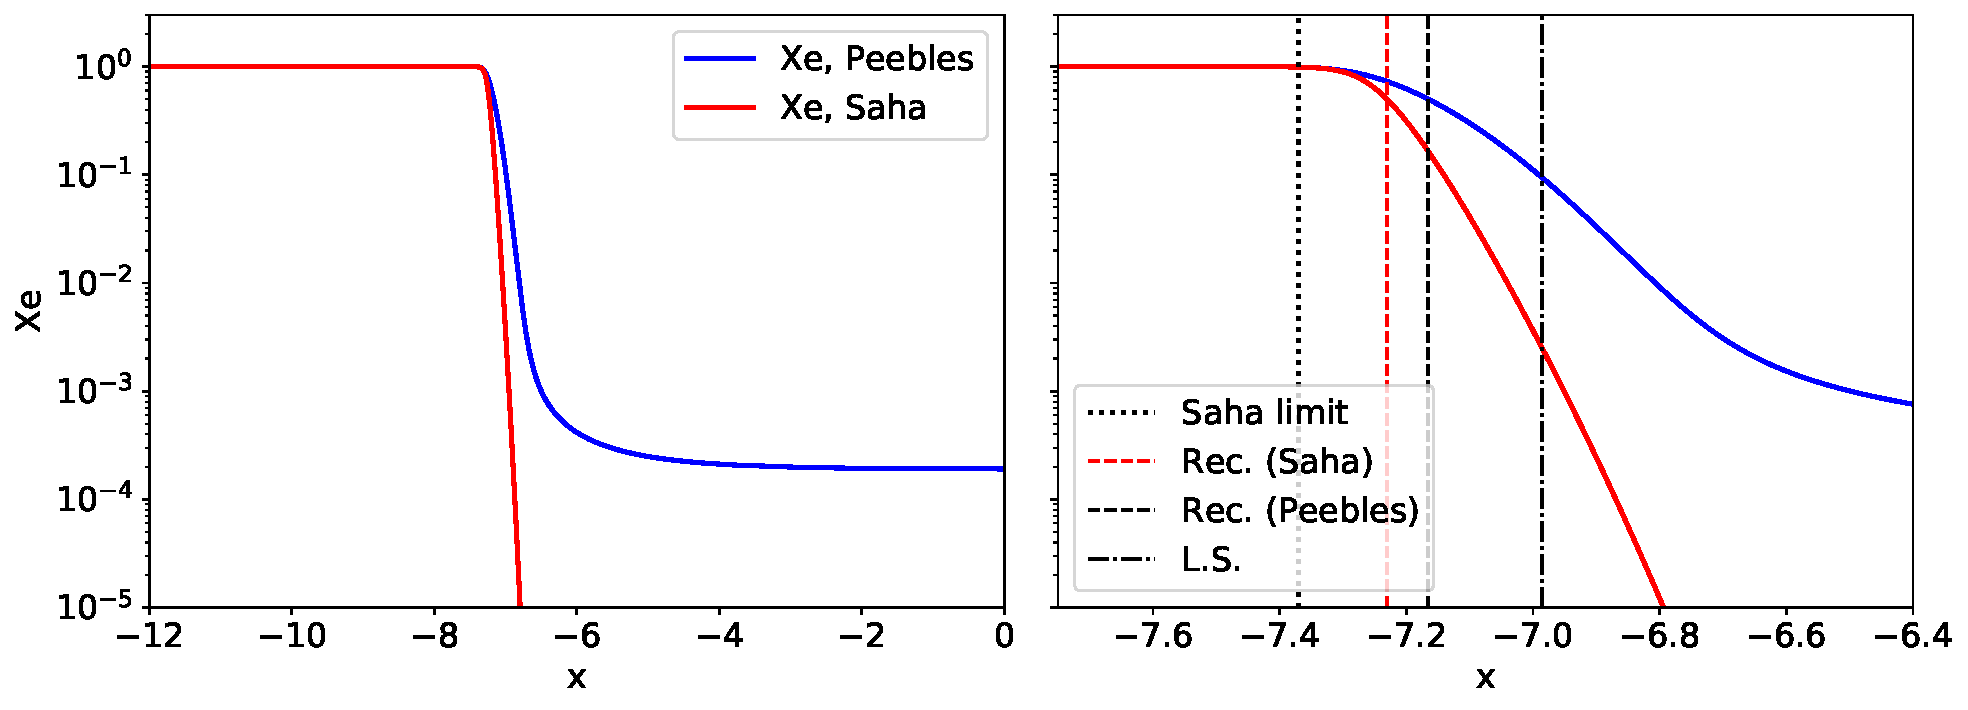
\includegraphics[scale=0.5]{../m2_figs/Xe.pdf}
    \caption{Figure showing the relative electron density as function of $x=\log{a}$, solved using the Saha equation only (red), and both the Saha and Peebles equation (blue), with a transition at $X_e = 0.99$. The right panel shows a zoomed in version, additionally showing the following events as vertical lines: 1) The Saha-Peebles transition limit, at $X_e = 0.99$. 2) The event of recombination, defined as $X_e = 0.5$, as calculated from the Saha equation only. 3) The event of recombination, as calculated by both the Saha and Peebles equation. 4) The surface of last scattering, defined as the point where $\tau = 1$ (see figure \ref{fig:tau}).}
    \label{fig:Xe}
\end{figure}

\begin{figure}[H]
    \centering
    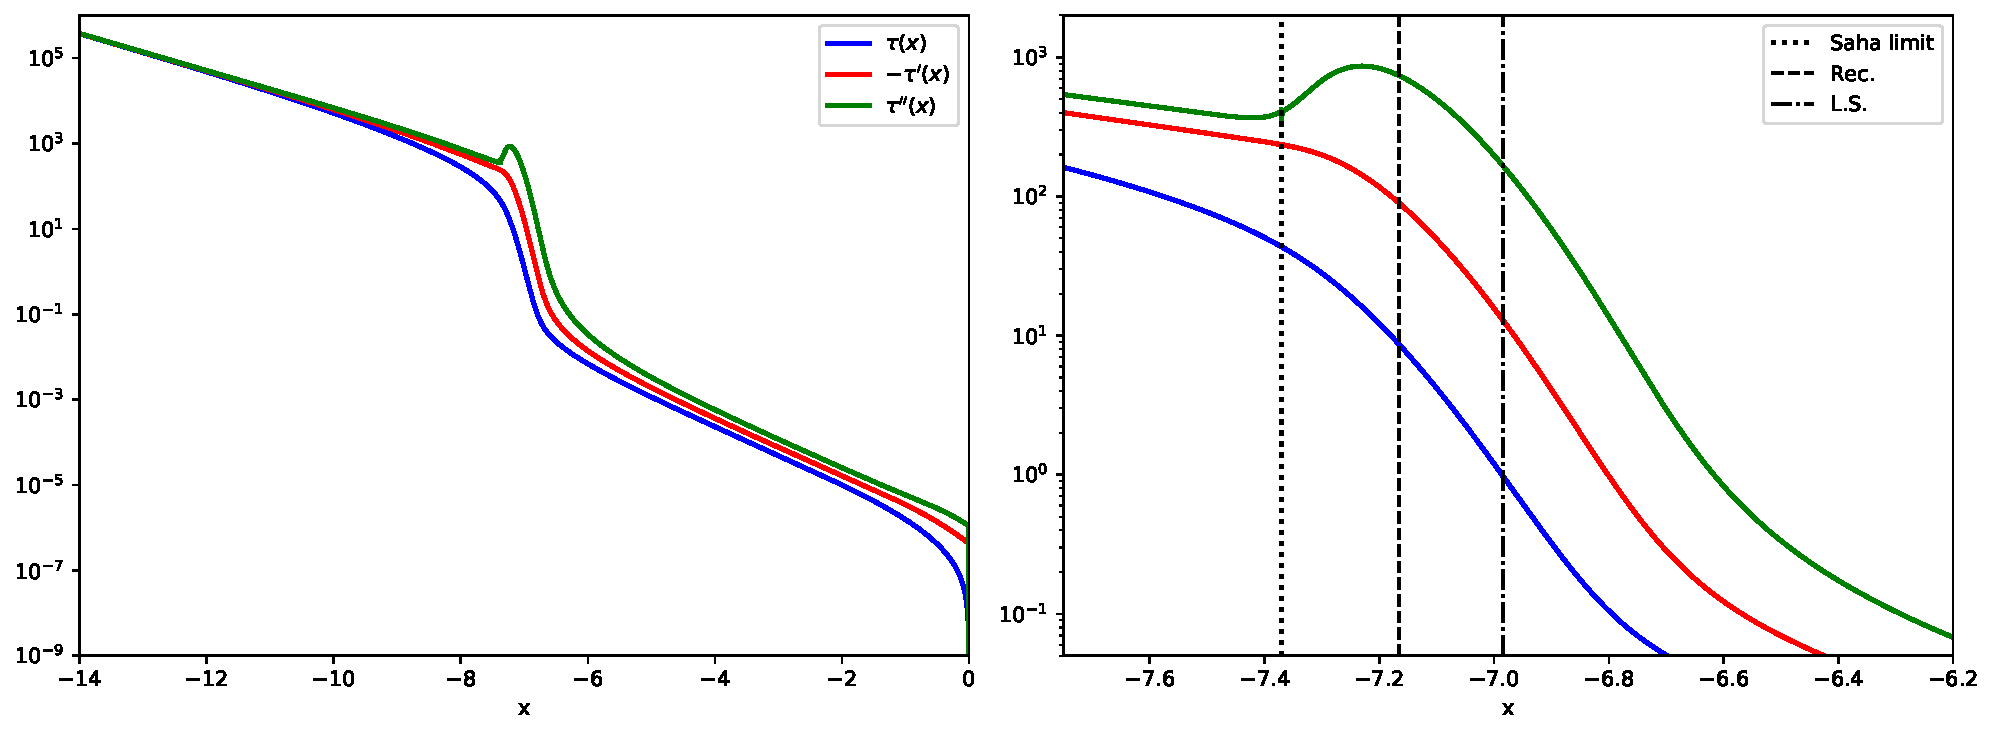
\includegraphics[scale=0.5]{../m2_figs/tau.pdf}
    \caption{Figure showing the optical depth $\tau(x)$, as well as its derivatives (with regards to $x$). The right panel shows a zoomed in version, in addition to vertical lines indicating events described in \ref{fig:Xe}.}
    \label{fig:tau}
\end{figure}

\begin{figure}[H]
    \centering
    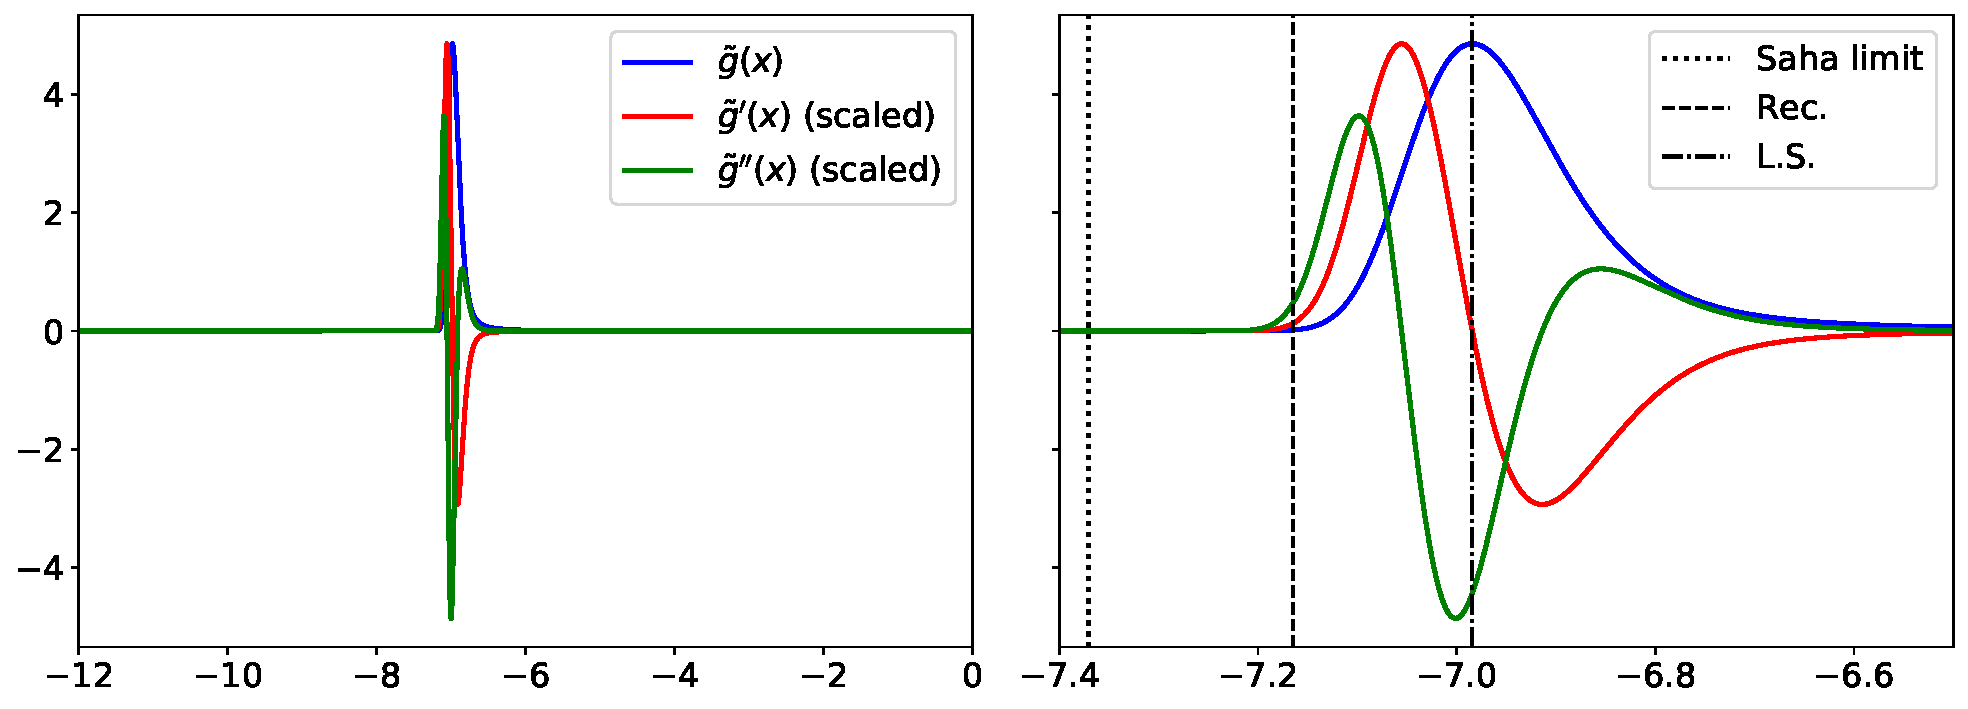
\includegraphics[scale=0.5]{../m2_figs/g_tilde.pdf}
    \caption{Figure showing the visibility function $\tilde{g}(x)$, and its derivatives (with regards to $x$). The first and second derivatives are scaled with factors of $0.0956$ and $0.0049$, respectively, such that their maxima coincide with that of $\tilde{g}(x)$. The right plot shows a zoomed in version, in addition to vertical lines indicating events described in \ref{fig:Xe}.}
    \label{fig:g_tilde}
\end{figure}

\appendix
\section{Dimensionality analysis}


\section{Saha-Peebles transition stability}
\begin{figure}[H]
    \centering
    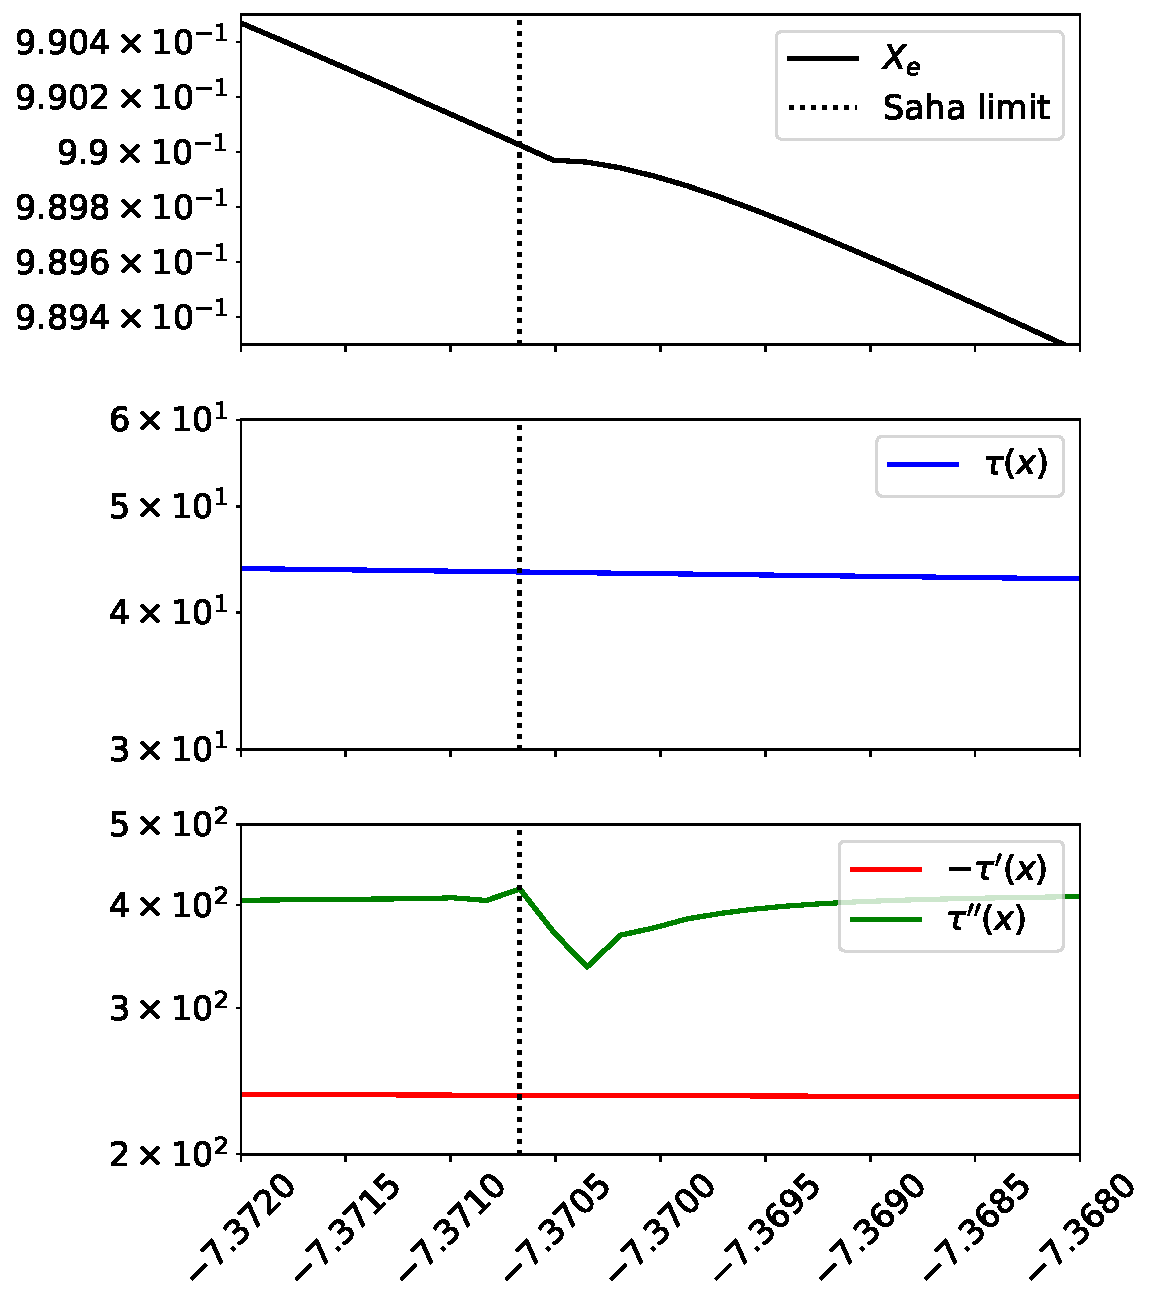
\includegraphics[scale=0.5]{../m2_figs/num_stab.pdf}
    \caption{}
    \label{fig:num_stab}
\end{figure}


\bibliography{ref}
\bibliographystyle{plain}



\end{document}